\documentclass[12pt]{article}

%% preamble: Keep it clean; only include those you need
\usepackage{amsmath}
\usepackage[margin = 1in]{geometry}
\usepackage{graphicx}
\usepackage{booktabs}
\usepackage{natbib}
\usepackage{adjustbox}
\usepackage{booktabs}
\usepackage[table]{xcolor}
\usepackage{svg}

% for space filling
\usepackage{lipsum}
% highlighting hyper links
\usepackage[colorlinks=true, citecolor=blue]{hyperref}


%% meta data

\title{Examining Various Statistical Methods in Predicting Loan Default}
\author{Chris Truedson\\
  Department of Statistics\\
  University of Connecticut
}

\begin{document}
\maketitle

\begin{abstract}
TBD  
\end{abstract}


\section{Introduction}
\label{sec:intro}

Approximately 22.7 million Americans have personal loans, 45 million have student loans, and 51.5 million households have mortgages with the vast majority of all these loans coming from banks and similar financial institutions. As such, it is crucial that these businesses are able to efficiently, accurately, and with the greatest level of optimization determine who it is safe to loan money to and who is likely to default. This is a practical business problem that is continuously being tinkered with to find new and better approaches. Many studies have took on the issue of using machine learning to predict whether a customer will default on a loan or not using various different methods like decision trees and random forests \citet{madaan2021loan}, KNN approaches \citet{lai2020loan}, and deep neural nets \citet{bayraci2019deep} to name a few.

% roadmap
The rest of the paper is organized as follows.
The data will be presented in Section~\ref{sec:data}.
The methods are described in Section~\ref{sec:meth}.
The results are reported in Section~\ref{sec:resu}.
A discussion concludes in Section~\ref{sec:disc}.


\section{Data}
\label{sec:data}

The data I'll be using will come from the \href{https://www.kaggle.com/datasets/nikhil1e9/loan-default}{Loan Default Prediction Dataset} on Kaggle. Itself is a dataset from a Coursera competition \href{https://www.coursera.org/projects/data-science-coding-challenge-loan-default-prediction}{Loan Default Prediction Challenge} featuring 255,347 observations and 18 variables with various demographic and financial data including but not limited to the borrowers age, their income, their education, their credit score, the loan amount, the type of loan, and various other metrics which provide a full picture of the loan, the borrower, and the borrower's financial situation.

\begin{table}[tbp]
  \caption{Structure of the Loan Default Dataset}
  \label{tab:rv}
\centering
\begin{tabular}{rrrp{3.5in}}
  \toprule
# & Column & Data Type & Description \\ 
  \midrule
0 & LoanID & object & A unique identifier for each loan \\ 
  1 & Age & int & The age of the borrower \\ 
  2 & Income & int & The annual income of the borrower \\ 
  3 & LoanAmount & int & The amount of money being borrowed \\ 
  4 & CreditScore & int & The credit score of the borrower \\ 
  5 & MonthsEmployed & int & The number of months the borrower has been employed \\ 
  6 & NumCreditLines & int & The number of credit lines the borrower has open \\ 
  7 & InterestRate & float & The interest rate for the loan \\ 
  8 & LoanTerm & int & The term length of the loan in months \\ 
  9 & DTIRatio & float & The Debt-to-Income ratio \\
  10 & Education & object & The highest level of education attained by the borrower (PhD, Master's, Bachelor's, High School) \\
  11 & EmploymentType & object & The type of employment status of the borrower (Full-time, Part-time, Self-employed, Unemployed) \\
  12 & MaritalStatus & object & The marital status of the borrower (Married, Divorced, Single) \\
  13 & HasMortgage & object & Whether the borrower has a mortgage (Yes/No) \\
  14 & HasDependents & object & Whether the borrower has dependents (Yes/No) \\
  15 & LoanPurpose & object & The purpose of the loan (Home, Business, Education, Auto, Other) \\
  16 & HasCoSigner & object & Whether the loan has a co-signer (Yes/No) \\
  17 & Default & object & Indicate whether the loan defaulted or not (0 = Did not default, 1 = Defaulted) \\ 
   \bottomrule
\end{tabular}
\end{table}

\begin{table}[htbp]
    \centering
    \caption{Summary Statistics}
    \small
    \setlength{\tabcolsep}{4pt}
    \begin{tabular}{l*{9}{@{\hspace{8pt}}p{0.5in}}}
        \toprule
        & Age & \hspace{4pt} Income & \hspace{12pt} Loan Amount & \hspace{8pt} Credit Score & Months Employed & Num Credit Lines & Interest Rate & Loan Term & DTI Ratio \\
        \midrule
        Mean & 43.49 & 82499.30 & 127578.87 & 574.26 & 59.54 & 2.50 & 13.49 & 36.03 & 0.50 \\
        Std & 14.99 & 38963.01 & 70840.71 & 158.90 & 34.64 & 1.12 & 6.64 & 16.97 & 0.23 \\
        Min & 18.00 & 15000.00 & 5000.00 & 300.00 & 0.00 & 1.00 & 2.00 & 12.00 & 0.10 \\
        25\% & 31.00 & 48825.50 & 66156.00 & 437.00 & 30.00 & 2.00 & 7.77 & 24.00 & 0.30 \\
        50\% & 43.00 & 82466.00 & 127556.00 & 574.00 & 60.00 & 2.00 & 13.46 & 36.00 & 0.50 \\
        75\% & 56.00 & 116219.00 & 188985.00 & 712.00 & 90.00 & 3.00 & 19.25 & 48.00 & 0.70 \\
        Max & 69.00 & 149999.00 & 249999.00 & 849.00 & 119.00 & 4.00 & 25.00 & 60.00 & 0.90 \\
        \bottomrule
    \end{tabular}
\end{table}

\begin{figure}[htbp]
    \centering
    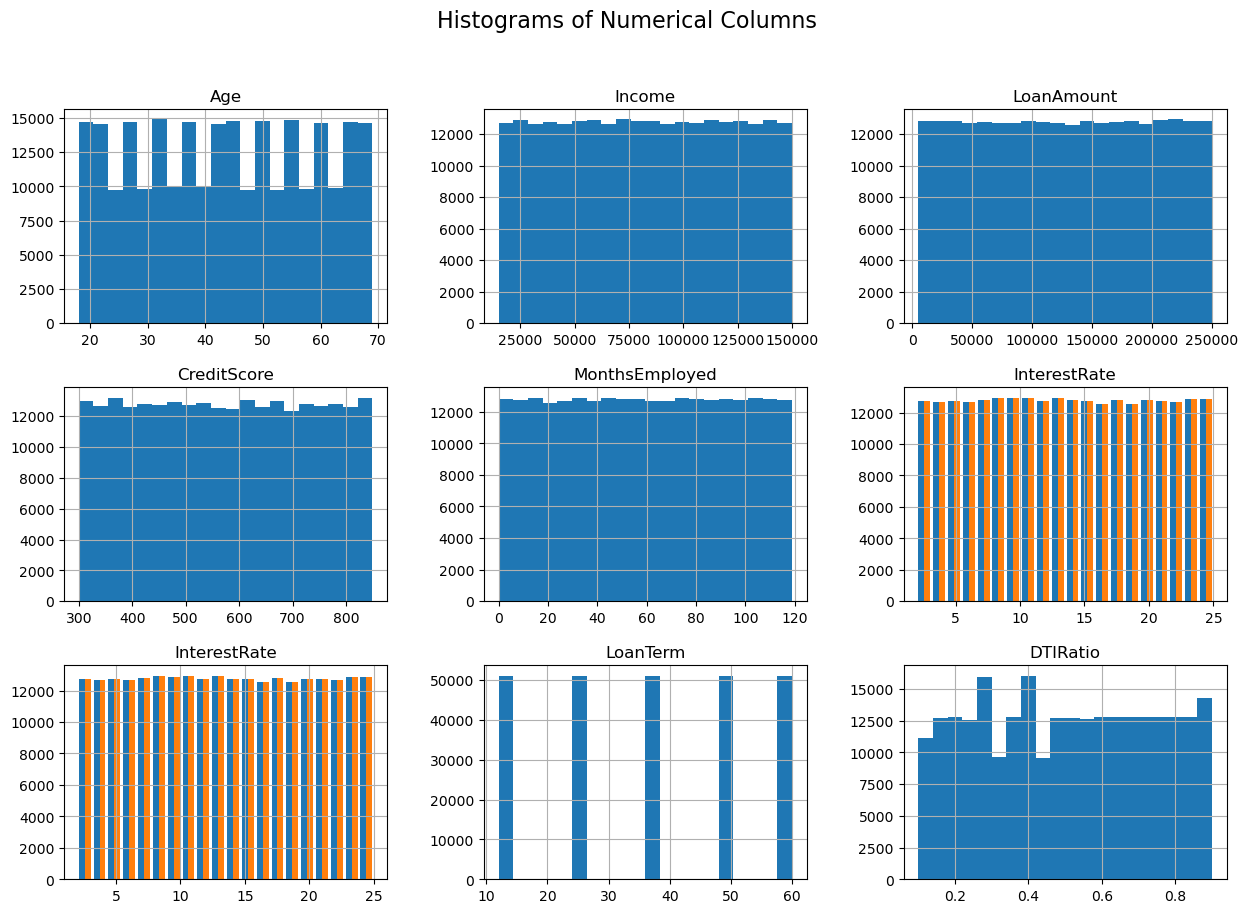
\includegraphics[width=\linewidth]{./code/Histogramsofnumericalcolumns.png}
    \caption{Distributions of all the numerical variables}
    \label{fig:numvarsdists}
\end{figure}

\begin{figure}[htbp]
    \centering
    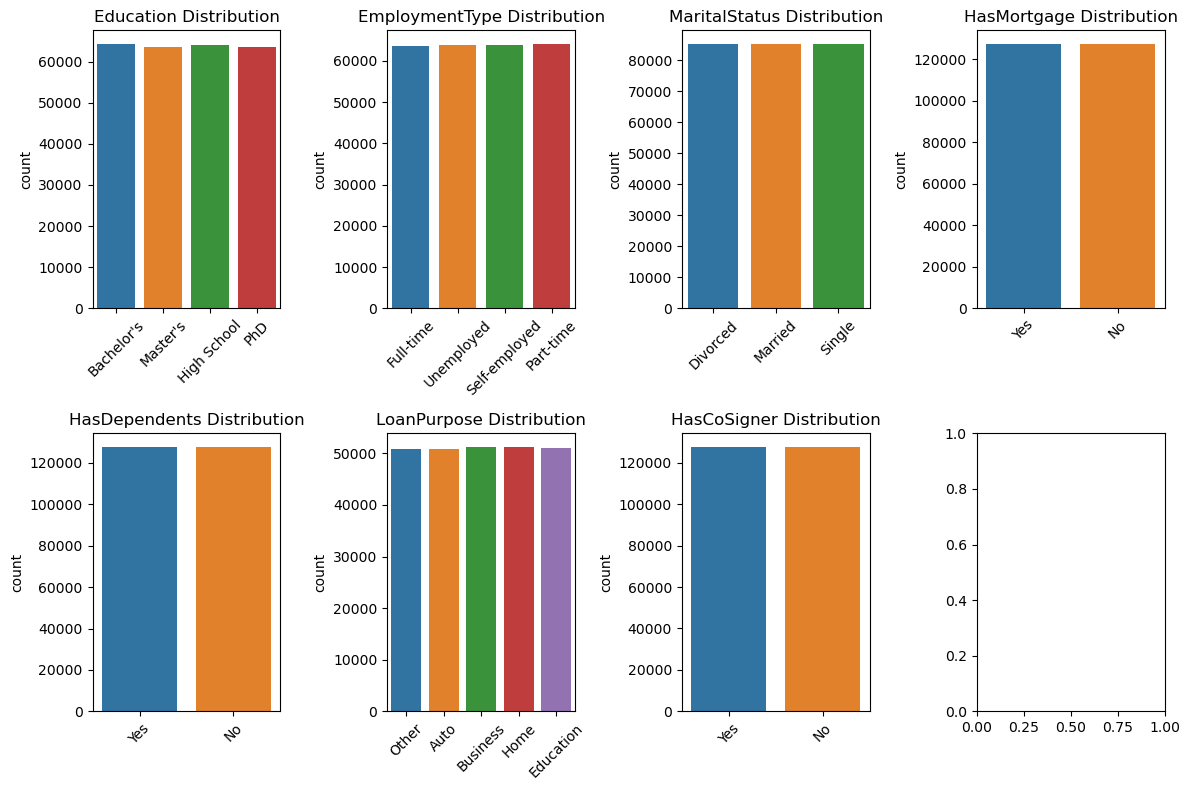
\includegraphics[width=\linewidth]{./code/categoricalvariablesdistributions.png}
    \caption{Distributions of all the categorical variables}
    \label{fig:catvarsdists}
\end{figure}

\begin{table}[htbp]
    \centering
    \caption{Correlation Matrix}
    \small
    \begin{adjustbox}{width=\textwidth}
    \begin{tabular}{l*{10}{@{\extracolsep{4pt}}c}}
        \toprule
        & Age & Income & LoanAmt & CScore & MEmployed & NCLines & IRate & LTerm & DTIRatio & Default \\
        \midrule
        Age & 1.0000 & -0.0012 & -0.0022 & -0.0005 & -0.0003 & -0.0009 & -0.0011 & 0.0003 & -0.0047 & -0.1678 \\
        Income & -0.0012 & 1.0000 & -0.0009 & -0.0014 & 0.0027 & -0.0020 & -0.0023 & -0.0010 & 0.0002 & -0.0991 \\
        LoanAmt & -0.0022 & -0.0009 & 1.0000 & 0.0013 & 0.0028 & 0.0008 & -0.0023 & 0.0025 & 0.0011 & 0.0867 \\
        CScore & -0.0005 & -0.0014 & 0.0013 & 1.0000 & 0.0006 & 0.0000 & 0.0004 & 0.0011 & -0.0010 & -0.0342 \\
        MEmployed & -0.0003 & 0.0027 & 0.0028 & 0.0006 & 1.0000 & 0.0013 & 0.0001 & -0.0012 & 0.0018 & -0.0974 \\
        NCLines & -0.0009 & -0.0020 & 0.0008 & 0.0000 & 0.0013 & 1.0000 & -0.0003 & -0.0002 & -0.0006 & 0.0283 \\
        IRate & -0.0011 & -0.0023 & -0.0023 & 0.0004 & 0.0001 & -0.0003 & 1.0000 & 0.0009 & 0.0006 & 0.1313 \\
        LTerm & 0.0003 & -0.0010 & 0.0025 & 0.0011 & -0.0012 & -0.0002 & 0.0009 & 1.0000 & 0.0023 & 0.0005 \\
        DTIRatio & -0.0047 & 0.0002 & 0.0011 & -0.0010 & 0.0018 & -0.0006 & 0.0006 & 0.0023 & 1.0000 & 0.0192 \\
        Default & -0.1678 & -0.0991 & 0.0867 & -0.0342 & -0.0974 & 0.0283 & 0.1313 & 0.0005 & 0.0192 & 1.0000 \\
        \bottomrule
    \end{tabular}
    \end{adjustbox}
\end{table}

\begin{figure}[htbp]
    \centering
    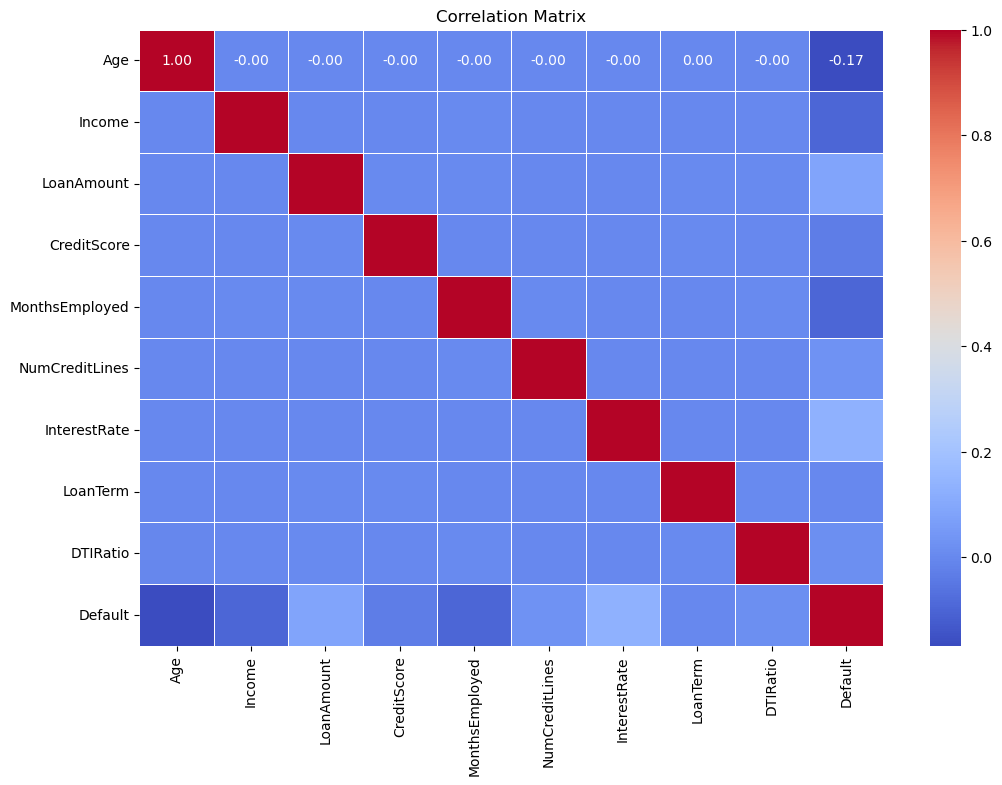
\includegraphics[width=\linewidth]{./code/fancycorrelationmatrix.png}
    \caption{Visualized correlation matrix}
    \label{fig:corrmatrix}
\end{figure}

\section{Methods}
\label{sec:meth}

Use this section to present the methodologies that will generate results by
analyzing the data. Suppose that the radius of a circle is $r$. Then its area is
\begin{equation}
  \label{eq:area}
  \pi r^2.
\end{equation}

Equation~\eqref{eq:area} is interesting.

Sometimes I don't want an equation to be numbered such as this one:
\[
  f(x) = \frac{1}{\sqrt{2\pi}} \exp\left( - \frac{x^2}{2} \right),
\]
which is the density of a standard normal variable.



\section{Results}
\label{sec:resu}

In order to find a model best suited to predicting default based on the provided data I ran several models such as a decision tree, a random forest, KNN, gradient boosting, various neural networks, adaboost, and bagging models. The data was split into a training and validation group of approximately 60\% training and 40\% validation (76,605 data points, with a significant imbalance between non-defaulters totaling 67,681 and defaulters making up the remaining 8,924.

\begin{table}[htbp]
    \centering
    \caption{Decision Tree Results}
    \begin{tabular}{lcccc}
        \toprule
        & Precision & Recall & F1-Score & Support \\
        \midrule
        0 & 0.90 & 0.88 & 0.89 & 67681 \\
        1 & 0.20 & 0.24 & 0.22 & 8924 \\
        Macro Avg & 0.55 & 0.56 & 0.55 & \\
        Weighted Avg & 0.82 & 0.80 & 0.81 & \\
        \midrule
        Accuracy & & & 0.80 & 76605 \\
        \bottomrule
    \end{tabular}
    \label{table:decisionTreeResults}
\end{table}

\begin{table}[htbp]
    \centering
    \caption{Decision Tree Confusion Matrix}
    \begin{tabular}{lcc}
        \toprule
        & Predicted 0 & Predicted 1 \\
        \midrule
        True 0 & 59373 & 8308 \\
        True 1 & 6825 & 2099 \\
        \bottomrule
    \end{tabular}
    \label{table:decisionTreeConfusionMatrix}
\end{table}

The decision tree model's results as shown above in Table \ref{table:decisionTreeResults} and Table \ref{table:decisionTreeConfusionMatrix} show the strengths and weaknesses of this particular model. For those classified as 0 (non-defaulters), the model shows high precision at 0.90, indicating that when it predicts a loan will not default, it is correct 90\% of the time. The recall for non-defaulters is slightly lower at 0.88, suggesting that the model correctly identifies 88\% of all actual non-default cases. The F1-score (a combination score balancing precision and recall) comes out to 0.89, suggesting strong performance among those that don't default.

By contrast, the model's performance on those classified as 1 (defaulters) is markedly weaker. The precision score for this group is only 0.20, meaning only 20\% of the instances predicted as defaults were actual defaults. The recall is slightly higher at 0.24, indicating that the model identifies 24\% of all actual default cases. The F1-score for this group comes out to 0.22, reflecting the models limited effectiveness in accurately predicting defaults.

The macro average, treating both groups equally into it's weight, shows moderate scores across precision, recall, and F1-scores (approximately 0.55), highlighting the disparity in model performance between the non-default group and the default group. The weighted average, considering this imbalance between groups, presents a better view (at around 0.81) due to it being heavily influenced by the models better performance on the far larger non-default group.

In looking closer at Table \ref{table:decisionTreeConfusionMatrix} the same results are further verified. Out of the 67,681 actual non-defaulters the model correctly identified 59,373 (True Negatives). However, it incorrectly predicted 8,308 as defaulters (False Positives). For the 8,924 actual defaulters, the model correctly predicted only 2,099 as defaulters (True Positives) but misclassified 6,825 as non-defaulters (False Negatives). Again further highlighting the models propensity towards false positives, showing how the model tends to fail in classifying defaulters.

The overall accuracy of the model comes out to 0.80, meaning it correctly predicts default correctly 80\% of the time across the entire validation data set. However, this high accuracy is partly misleading due to the significant group imbalance we observe with the model being far more effective at identifying non-defaulters than defaulters.

\begin{table}[htbp]
    \centering
    \caption{Random Forest Results}
    \begin{tabular}{lcccc}
        \toprule
        & Precision & Recall & F1-Score & Support \\
        \midrule
        0 & 0.89 & 1.00 & 0.94 & 67681 \\
        1 & 0.71 & 0.03 & 0.06 & 8924 \\
        Macro Avg & 0.80 & 0.51 & 0.50 & \\
        Weighted Avg & 0.87 & 0.89 & 0.84 & \\
        \midrule
        Accuracy & & & 0.89 & 76605 \\
        \bottomrule
    \end{tabular}
    \label{table:randomForestResults}
\end{table}

\begin{table}[htbp]
    \centering
    \caption{Random Forest Confusion Matrix}
    \begin{tabular}{lcc}
        \toprule
        & Predicted 0 & Predicted 1 \\
        \midrule
        True 0 & 67565 & 116 \\
        True 1 & 8642 & 282 \\
        \bottomrule
    \end{tabular}
    \label{table:randomForestConfusionMatrix}
\end{table}

The random forest model's results as shown above in Table \ref{table:randomForestResults} and Table \ref{table:randomForestConfusionMatrix} show the many of the same strengths and weaknesses we saw with the previous decision tree model. For those classified as 0 (non-defaulters), the model has a high level precision at 0.89 and an excellent recall of 1.00, which lead in turn to an F1-score of 0.94. These values indicate that the model is almost perfect in identifying non-default cases but has a slight tendency to mislabel a few default cases as non-defaults.

Among those classified as 1 (defaulters) the precision is 0.71, suggesting that when the model predicts a default, it is correct 71\% of the time, a fairly good percentage. However, the recall is extremely low at 0.03, meaning the model identifies only 3\% of the actual default cases present. The F1-score for this group is just 0.06, reflecting the model's poor performance in predicting defaults.

The macro average scores are lower (0.80 precision, 0.89 recall, and 0.50 for F1-score) suggesting there's a significant imbalance in the model's ability to predict non-defaulters and defaulters as seen previously. The weighted average scores (0.87 precision, 0.89 recall, and 0.84 F1-score) are higher, this reflects the influence of the model's strong performance in the majority group of non-defaulters.

In looking closer at Table \ref{table:randomForestConfusionMatrix} again the results above are verified. Out of the 67,681 actual non-defaulters 67,565 were correctly identified, with only 116 incorrectly predicted as defaulters. On the other hand of the 8,924 actual defaulters, only 282 were correctly identified, while a significant number 8,642, were incorrectly labeled as non-defaulters.

The random forest model appears to demonstrate strong performance in predicting non-defaults, evidenced by the high precision, recall, and F1-score for group 0, as well as the large number of true negatives. However, its ability to identify actual default cases is pretty terrible, as shown by the extremely low reacall and F1-score for group 1, and the high number of false negatives.

The overall model accuracy is 0.89, which, while high, is largely driven by its success in correctly predicting the majority class of non-defaulters and masks the model's severe limitations in accurately identifying default cases.

\begin{table}[htbp]
    \centering
    \caption{KNN Results}
    \begin{tabular}{lcccc}
        \toprule
        & Precision & Recall & F1-Score & Support \\
        \midrule
        0 & 0.89 & 0.98 & 0.93 & 67681 \\
        1 & 0.26 & 0.04 & 0.07 & 8924 \\
        Macro Avg & 0.57 & 0.51 & 0.50 & \\
        Weighted Avg & 0.81 & 0.87 & 0.83 & \\
        \midrule
        Accuracy & & & 0.87 & 76605 \\
        \bottomrule
    \end{tabular}
    \label{table:kNNResults}
\end{table}

\begin{table}[htbp]
    \centering
    \caption{KNN Confusion Matrix}
    \begin{tabular}{lcc}
        \toprule
        & Predicted 0 & Predicted 1 \\
        \midrule
        True 0 & 66639 & 1042 \\
        True 1 & 8553 & 371 \\
        \bottomrule
    \end{tabular}
    \label{table:kNNConfusionMatrix}
\end{table}

The k nearest number model's results as shown above in Table \ref{table:kNNResults} and Table \ref{table:kNNConfusionMatrix} show a continuation of the results we've seen in the previous two models. For those classified as 0 (non-defaulters) the model shows strong performance with a precision of 0.89 and an even higher recall of 0.98, culminating with an F1-score of 0.93. This indicates the model is highly effective in identifying non-default cases, with a tendency to misclassify certain default cases as non-defaults.

For defaulters, the model's precision is low at 0.26, meaning only about 26\% of the instances predicted as default are actual defaults. The recall is far lower at 0.04 meaning the model only correctly identifies a mere 4\% of all actual default cases. The F1-score reflects this at 0.07, highlighting the poor performance in predicting defaults.

The macro average scores are moderate (0.57 precision, 0.51 recall, and 0.50 F1-score), further showing the significant disparity between predicting between non-defaulters and defaulters. The weighted average scores (0.81 precision, 0.87 recall, and 0.83 F1-score) are higher, but is merely reflecting the models better performance among the majority group.

The confusion matrix shown in Table \ref{table:kNNConfusionMatrix} verifies these findings as of the 67,681 actual non-defaulters, 66,639 were correctly identified, with 1,042 incorrectly labeled as defaulters. Out of the 8,924 actual defaulters, only 371 were correctly identified, with a substantial 8,553 misclassified as non-defaulters. 

The KNN model demonstrates a strong ability to identify non-defaults as seen with the other models and evidenced by its high precision, recall, and F1-score for the non-defaulter group with a substantial amount of true negatives. However, its capacity for to accurately identify default cases is weak shown by the aforementioned metrics and the amount of false negatives.

The overall model accuracy score stands at 0.87, largely influenced by its effectiveness in predicting the far more prevalent in the data set non-defaulter group. 

\begin{table}[htbp]
    \centering
    \caption{Gradient Boosting Results}
    \begin{tabular}{lr}
        \toprule
        Model & Accuracy \\
        \midrule
        XGBoost & 0.8865 \\
        LightGBM & 0.8866 \\
        CatBoost & 0.8860 \\
        \bottomrule
    \end{tabular}
    \label{table:gradientBoostingResults}
\end{table}

The gradient boosting models results shown above in Table \ref{table:gradientBoostingResults} suggest much of the same results as previous. Of the three gradient boosting model approaches attempted the accuracy results are very similar among all the models and suggest a high degree of accuracy. With that said, these models suffere from the same flaws as the models reviewed previously in that they are good at predicting among the majority group of non-defaulters but struggle in predicting defaults correctly.

Looking firstly at the XGBoost (Extreme Gradient Boosting) model we see an accuracy of 0.8865. An accuracy of 88.65\% indicates that the model correctly predicted the loan default status for this percentage of cases over the validation data set.

Next, the LightGBM (Light Gradient Boosting Model) we see an accuracy just above that of the XGBoost model and the highest of the three gradient boost models tested. An accuracy of 88.66\% indicates that the model correctly predicted the loan default status for this percentage of cases over the validation data set.

Finally, the CatBoost (Categorical Boost) model is marginally lower than the other two but still very close to all the others tested indicating a high level of predictability. An accuracy of 88.60\% indicates that the model correctly predicted the loan default status for this percentage of cases over the validation data set.

\begin{table}[htbp]
    \centering
    \caption{FF Neural Network Results}
    \begin{tabular}{cccccc}
        \toprule
        NumHiddenLayers & NumUnits & DropoutRate & Accuracy \\
        \midrule
        \rowcolor{green!25}2 & 32 & 0.3 & 0.887742 \\
        2 & 32 & 0.5 & 0.887253 \\
        2 & 32 & 0.7 & 0.885628 \\
        2 & 64 & 0.3 & 0.887214 \\
        2 & 64 & 0.5 & 0.887037 \\
        2 & 64 & 0.7 & 0.887351 \\
        2 & 128 & 0.3 & 0.887292 \\
        2 & 128 & 0.5 & 0.887449 \\
        2 & 128 & 0.7 & 0.886352 \\
        3 & 32 & 0.3 & 0.885040 \\
        3 & 32 & 0.5 & 0.884570 \\
        3 & 32 & 0.7 & 0.884472 \\
        3 & 64 & 0.3 & 0.885451 \\
        3 & 64 & 0.5 & 0.884472 \\
        3 & 64 & 0.7 & 0.884472 \\
        3 & 128 & 0.3 & 0.885941 \\
        3 & 128 & 0.5 & 0.884472 \\
        3 & 128 & 0.7 & 0.884472 \\
        4 & 32 & 0.3 & 0.884472 \\
        4 & 32 & 0.5 & 0.884472 \\
        4 & 32 & 0.7 & 0.884472 \\
        4 & 64 & 0.3 & 0.884511 \\
        4 & 64 & 0.5 & 0.884531 \\
        4 & 64 & 0.7 & 0.884472 \\
        4 & 128 & 0.3 & 0.884668 \\
        4 & 128 & 0.5 & 0.884511 \\
        4 & 128 & 0.7 & 0.884472 \\
        \bottomrule
    \end{tabular}
    \label{table:fFNeuralNetworkResults}
\end{table}

The feedforward neural network model results with variations for tuning shown above in Table \ref{table:fFNeuralNetworkResults} shows much of the same with regards to accuracy levels, strengths, and weaknesses. This neural network was run under a variety of configurations varying the number of hidden layers, the number of units/neurons, and the dropout rate. The primary metric being used to evaluate the models being their accuracy.

The accuracies of the models range from 88.47\% to 88.77\%. These values indicate the proportion of the total number of predictions that were correct. The highest accuracy achieved was 88.7742\%, with a configuration of 2 hidden layers, 32 units, and a dropout rate of 0.3. 

Generally it appeared models with 2 hidden layers performed marginally better than those with 3 or 4 layers, suggesting that additional complexity does not necessarily translate to better performance under this particular data set. The varitaion in accuracy across different dropout rates is relatively small, indicating that the models are somewhat robust to this parameter. However, the highest accuracy is achieved with a lower dropout rate (0.3), suggesting that a higher drop out rate leading to too much regularization might be detrimental in this case.

The FFNN models demonstrate good performance in predicting loan defaults. However, as models above due to the nature of the data set much of the accuracy is skewed due to the models being far better at predicting the majority group of non-default over than the default group.

\begin{table}[htbp]
    \centering
    \caption{Neural Network Results}
    \begin{tabular}{lc}
        \toprule
        Model & Accuracy \\
        \midrule
        FFNN & 0.8877 \\
        CNN & 0.8878 \\
        RNN & 0.8872 \\
        \bottomrule
    \end{tabular}
    \label{table:neuralNetworkResults}
\end{table}

The nerual network results shown above in Table \ref{table:neuralNetworkResults} shows the results for a variety of nerual network types, taking the best feedforward results from Table \ref{table:fFNeuralNetworkResults}, and adding results for a CNN (Convolutional Neural Network), and a RNN (Recurrent Neural Network) model.

Looking at the models not previously discussed starting with the CNN we sigh a marginally higher accuracy score for this model of 88.78\% a 0.01\% improvement over the FFNN. The RNN was the lowest scoring of the pact for neural network models with an accuracy score of 88.72\%.

All three neural network models demonstrate comparable and high accuracy in predicting loan default outcomes but with little overall difference among them. These accuracy scores aren't the whole picture as discussed previously as all these models are seeing misleadingly high accuracy scores due to the large nature of non-defaults present in the data set and the propensity of the models to choose non-default.

\begin{table}[htbp]
    \centering
    \caption{Adaboost Results}
    \begin{tabular}{lcccc}
        \toprule
        & Precision & Recall & F1-Score & Support \\
        \midrule
        0 & 0.89 & 0.99 & 0.94 & 45170 \\
        1 & 0.56 & 0.08 & 0.15 & 5900 \\
        Macro Avg & 0.73 & 0.54 & 0.54 & 51070 \\
        Weighted Avg & 0.85 & 0.89 & 0.85 & 51070 \\
        \midrule
        Accuracy & & & 0.89 & 51070 \\
        \bottomrule
    \end{tabular}
    \label{table:adaboostResults}
\end{table}

\begin{table}[htbp]
    \centering
    \caption{Adaboost Confusion Matrix}
    \begin{tabular}{lcc}
        \toprule
        & Predicted 0 & Predicted 1 \\
        \midrule
        True 0 & 44782 & 388 \\
        True 1 & 5403 & 497 \\
        \bottomrule
    \end{tabular}
    \label{table:adaboostConfusionMatrix}
\end{table}

The Adaboost model's results as shown above in Table \ref{table:adaboostResults} and Table \ref{table:adaboostConfusionMatrix} show much the same with regards to what we've seen repeatedly in regards to modeling this data set, however, there does appear to be some marginal improvement in some metrics. As is expected at this point the model shows strong performance for non-defaulters with a precision of 0.94 and a very high recall of 0.99 for a combined F1-score of 0.94. This all indicates the model is highly effective in identifying non-default cases, with a very low rate of misclassifying non-defaulters.

For defaulters, the model's precision is moderate at 0.56, suggesting that when it predicts default, it is correct about 56\% of the time. However, it's recall is quite low at 0.08, meaning that the model correctly identifies only 8\% of actual default cases. The F1-score of 0.15 reflects the poor performance among this group.

The macro average scores are all around 0.54, indicating a disparity as seen throughout with regards to the models ability to predict among the non-defaulters and defaulters. The weighted average scores are all around 0.85 and are influenced by the model's much stronger performance among the prevalent group of non-defaulters.

The confusion matrix shown in Table \ref{table:adaboostConfusionMatrix} further confirms the results. Out of 45,170 actual non-defaulters, 44,782 were correctly identified, with 388 incorrectly predicted as defaulters. Of the 5,900 actual defaulters only 497 were correctly identified meaning 5,403 were misidentified (False Negatives).

The Adaboost model sees strong performance in non-defaulters as has been the trend throughout models. The overall accuracy is listed as 0.89, which, while high is misleading due to the nature of the data set as previously discussed.

\begin{table}[htbp]
    \centering
    \caption{Bagging Results}
    \begin{tabular}{lcccc}
        \toprule
        & Precision & Recall & F1-Score & Support \\
        \midrule
        0 & 0.89 & 1.00 & 0.94 & 45170 \\
        1 & 0.75 & 0.02 & 0.04 & 5900 \\
        Macro Avg & 0.82 & 0.51 & 0.49 & 51070 \\
        Weighted Avg & 0.87 & 0.89 & 0.84 & 51070 \\
        \midrule
        Accuracy & & & 0.89 & 51070 \\
        \bottomrule
    \end{tabular}
    \label{table:boostingResults}
\end{table}

\begin{table}[htbp]
    \centering
    \caption{Bagging Confusion Matrix}
    \begin{tabular}{lcc}
        \toprule
        & Predicted 0 & Predicted 1 \\
        \midrule
        True 0 & 45125 & 45 \\
        True 1 & 5765 & 135 \\
        \bottomrule
    \end{tabular}
    \label{table:boostingConfusionMatrix}
\end{table}

Finally as has become the trend the Boosting model's results shown above in Table \ref{table:boostingResults} and Table \ref{table:boostingConfusionMatrix} show the story we've seen repeatedly in modeling this data set. The model demonstrates strong performance for non-defaulters, with a precision of 0.89 and a near perfect recall of 1.00, for a F1-score of 0.94. The model has shown to be highly effective in identifying non-default cases and has minimal rate of misclassification for default cases as non-defaults.

For defaulters, the model has a moderately strong precision of 0.75 meaning when it predicts default it's largely correct. With that said the recall is terrible at 0.02, meaning only 2\% of actual default cases are correctly identified as such. All combining for an F1-score of 0.04 to highlight this performance issue.

The macro average scores are 0.82 precision, 0.51 recall, and 0.49 for F1-score, showing the imbalance in the data we've seen throughout models. The weighted average scores are 0.87 precision, 0.89 recall, and 0.84 for F1-score, these higher scores mask the poor performance among predicting defaulters due to the data set's larger sample of non-defaulters.

The confusion matrix shown in Table \ref{table:boostingConfusionMatrix} adds further to the results already discussed. Out of the 45,170 actual non-defaulters 45,125 were correctly identified and just 45 were incorrectly predicted as defaulters. Whereas out of 5,900 actual defaulters only 135 were correctly identified, with the significant majority being misclassified as non-defaulters highlighting the very large false negative rate.

The bagging model shows good performance in non-defaulters as nearly every other model does, largely influenced by the nature of the data set it was trained on. The overall accuracy of the model comes out to 0.89, driven by the imbalance in the data set.

\section{Discussion}
\label{sec:disc}

The most challenging parts of the proposed work will be fitting and tuning each of the models. While straightforward in building them each model will require tuning using a variety of techniques. More difficult still will be testing more models than just those that have been proposed with perhaps even more specialized and advanced machine learning models like deep neural networks and even extreme gradient boosting as discussed in \citet{lai2020loan}. 
\par The limitations of my work are twofold. With regards to my first aim of finding the most important variables, the dataset I'm working with contains 18 of probably the most common types of variables used in this setting however, other critical variables may be missing making my work in finding the most significant variables and seeing if they change with the type of loan bounded. In regards to my second aim of finding the "best" model, there's many limitations such as I won't be testing ALL possible models, instead I'll only be testing the most common and relatively simple with the possibility for some less employed more advanced models to be tested as well. Additionally, the dataset while "large" at approximately 250,000 observations businesses could be working with datasets magnitude of this size which if the models prove to all be very effective with very minor accuracy changes between them could see a shift in a much larger dataset of the "best" model.  
\par Overall, I expect this project to go relatively smoothly as the project while it has complex components depending on the models employed and the level of tuning at the most base level is relatively straightforward. If things do go wrong for whatever reason there were multiple other datasets I found with similar variables and looking at default prediction which could be used to replace or even compliment potentially my current dataset.

\bibliography{refs}
\bibliographystyle{mcap}

\end{document}